\begin{multicols}{2}
\large	
	Em 1958, o físico americano William Higinbotham (1910-1994) cria o primeiro videogame do mundo: \textbf{Tenis for Two}.
	
	\begin{flushright}
		\normalsize Fonte: \href{https://warpzone.me/primeiro-videogame-do-mundo-comemora-60-anos/}{https://warpzone.me/primeiro-videogame-do-mundo-comemora-60-anos/}
	\end{flushright}

\vfill\null
\columnbreak

	\begin{center}
		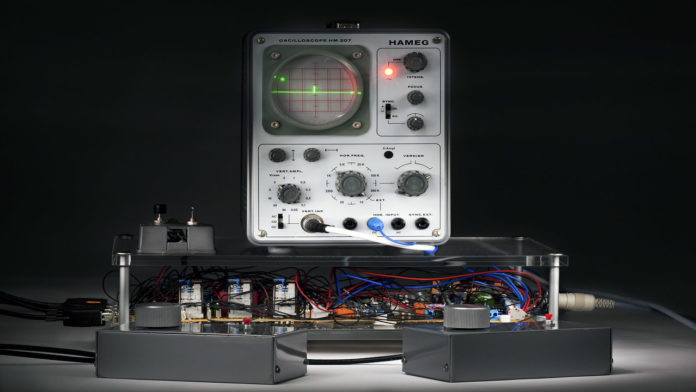
\includegraphics[width=\linewidth]{./IMG/tenis1-696x392.jpg}
	\end{center}

\vfill\null
\columnbreak

\begin{center}
	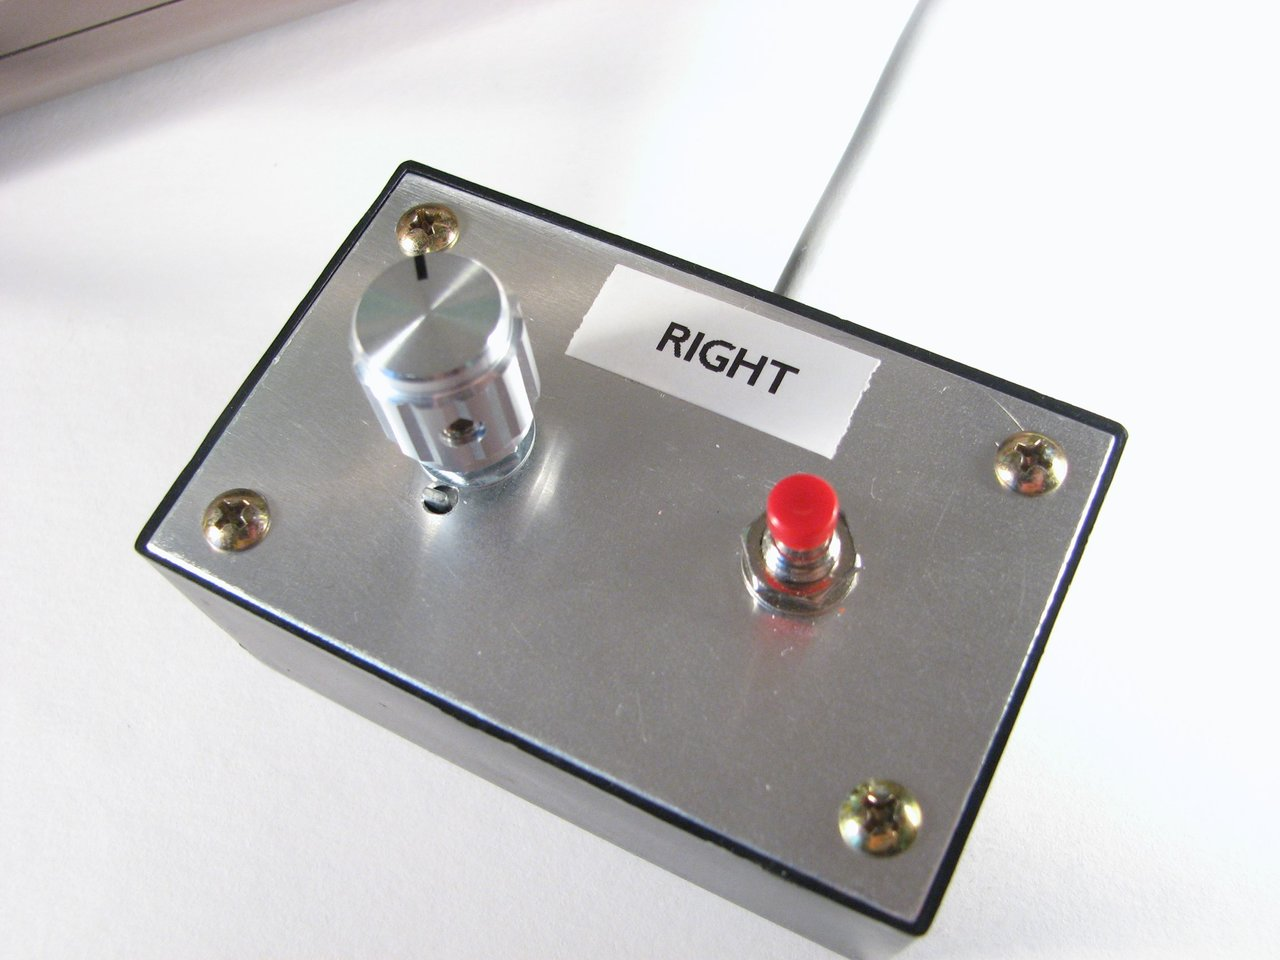
\includegraphics[width=\linewidth]{./IMG/tenis2.jpg}
\end{center}


\vfill\null
\columnbreak

\begin{center}
	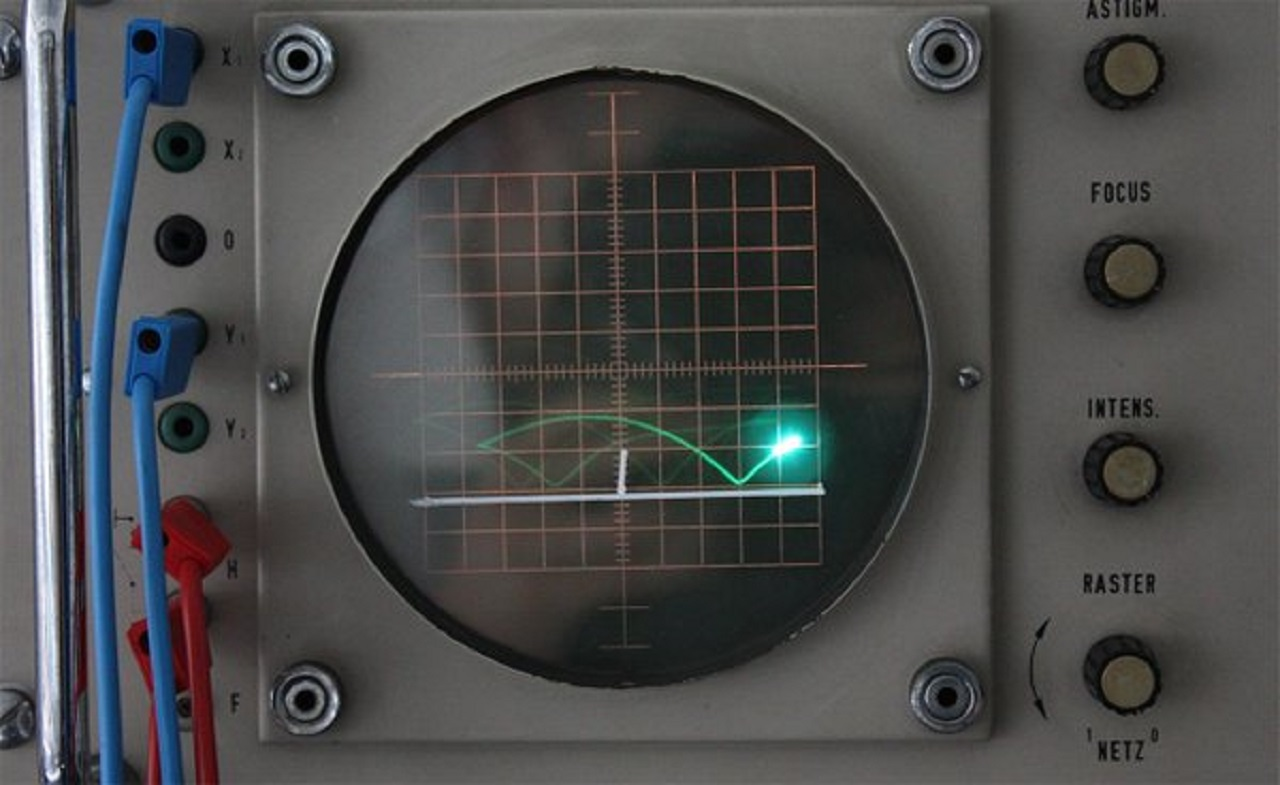
\includegraphics[width=\linewidth]{./IMG/tenis-3.jpg}
\end{center}

\vfill\null
\columnbreak


\Large \textbf{Atari}: a lenda!

	\begin{center}
	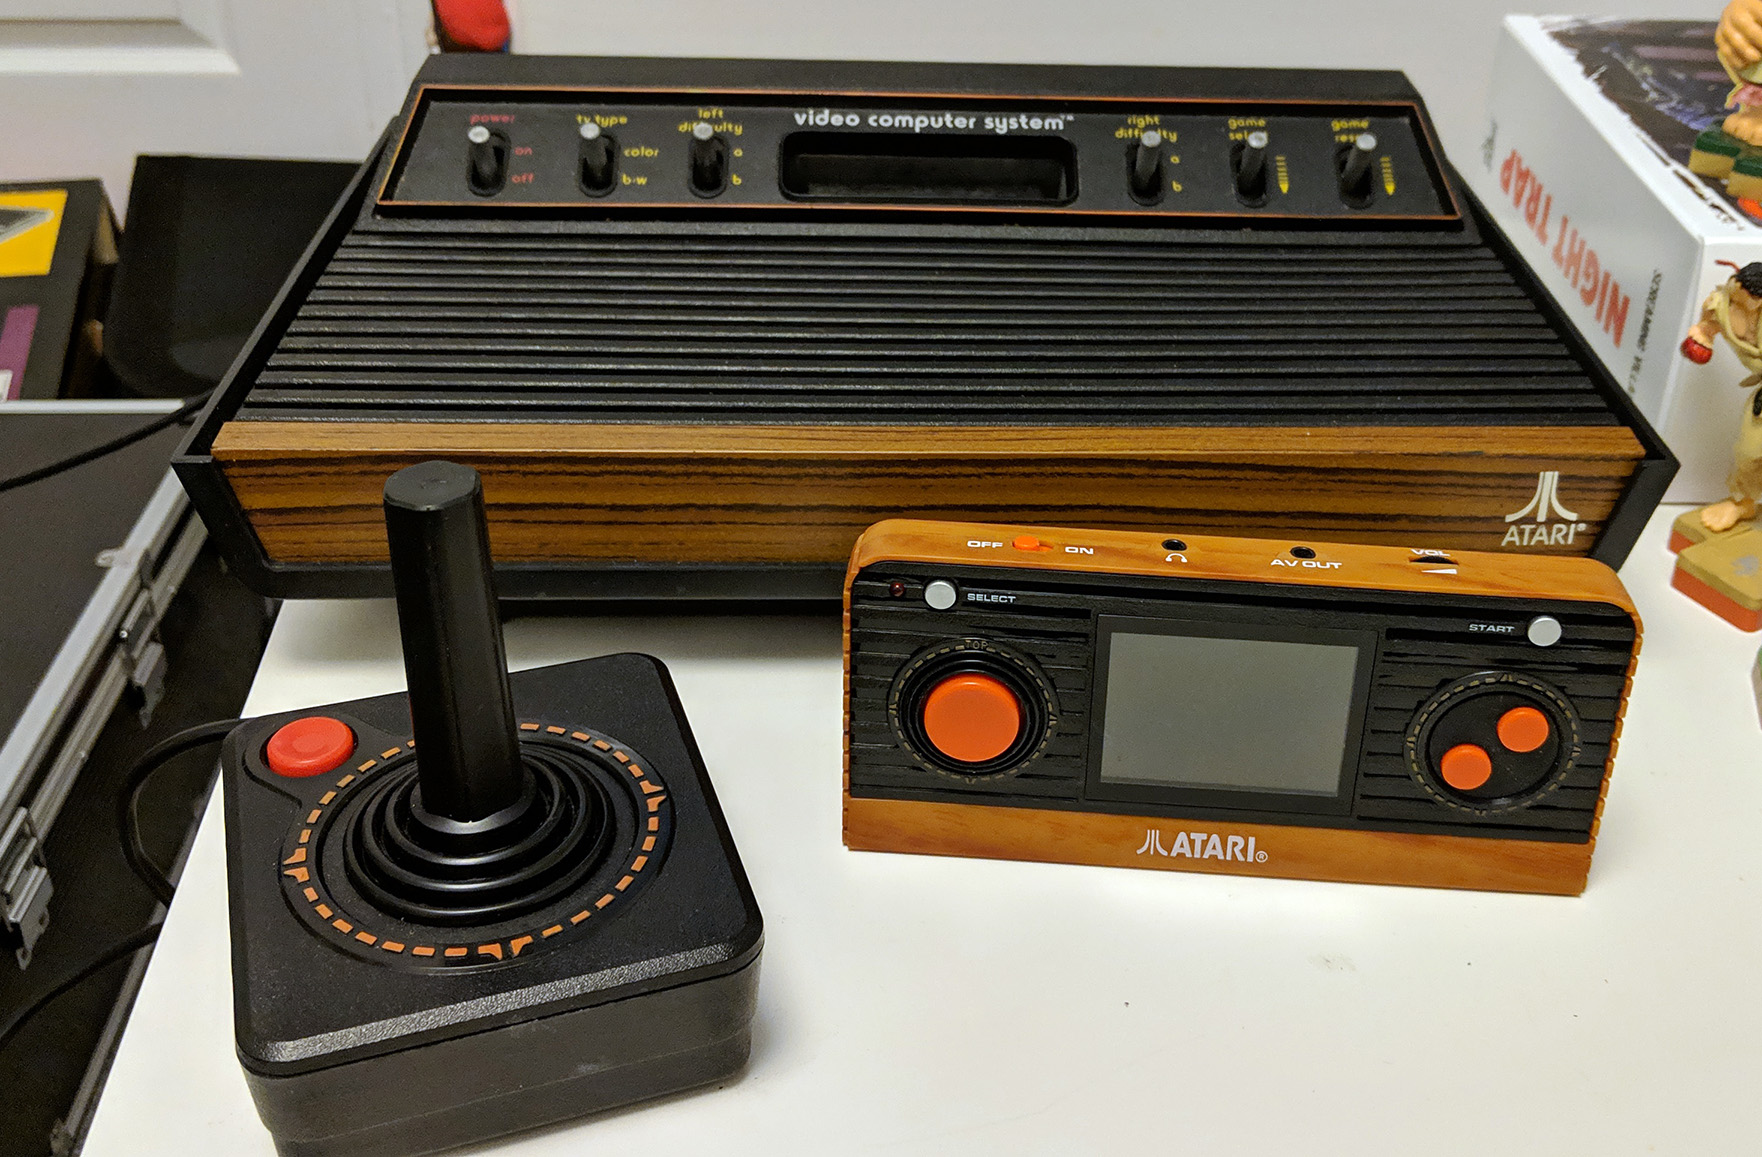
\includegraphics[width=\linewidth]{./IMG/atari-2600-handheld-pic3-2222881701.jpg}
\end{center}

\vfil\null
\columnbreak

	\begin{center}
	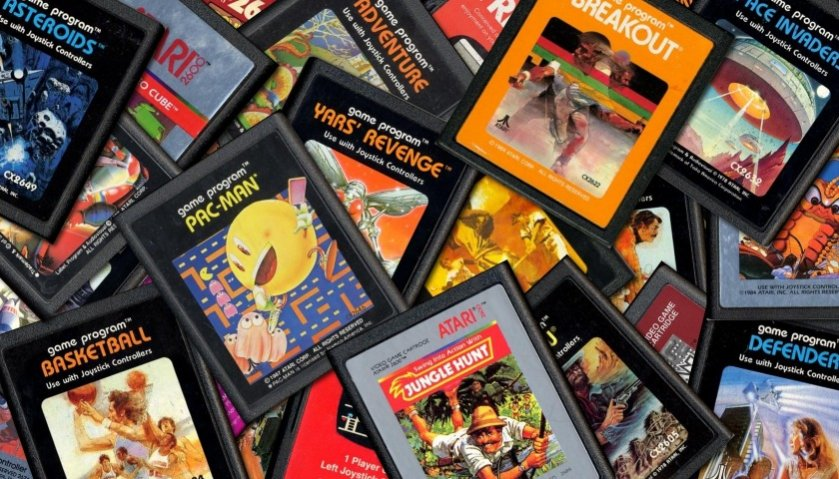
\includegraphics[width=\linewidth]{./IMG/ATARI-1124950375.jpg}
\end{center}

\vfil\null
\pagebreak

\pagecolor{black}
{\color{white}Enduro}

	\begin{center}
	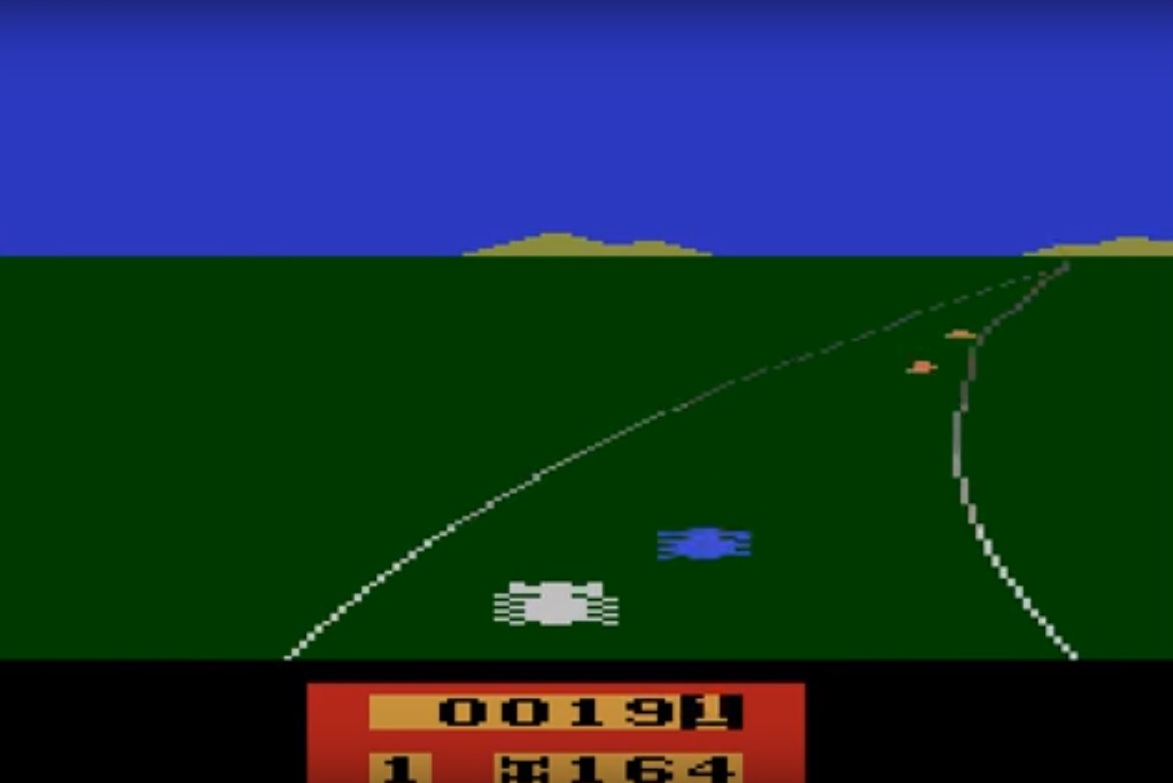
\includegraphics[width=\linewidth]{./IMG/enduroatari2600image1111.jpg}
\end{center}

\vfil\null
\columnbreak

{\color{white}Pacman}
\begin{center}
	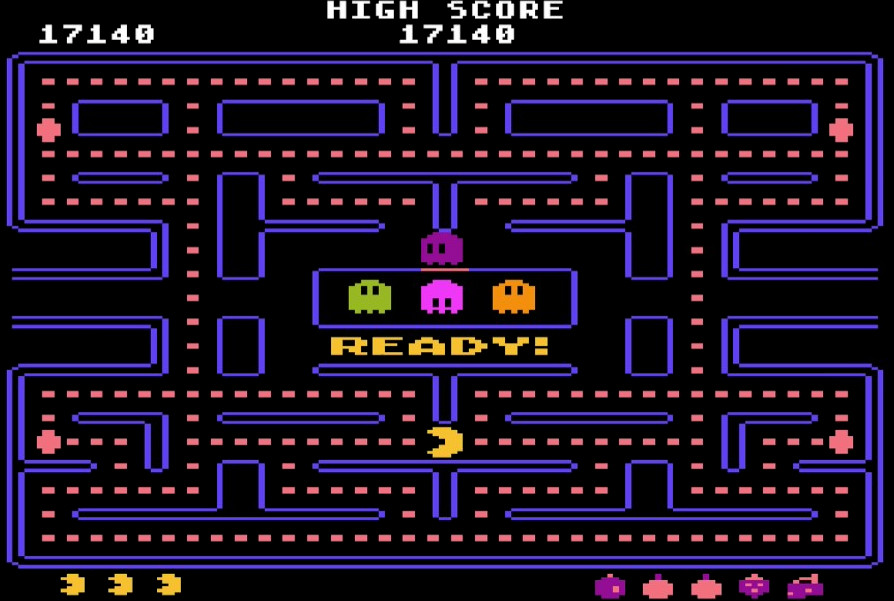
\includegraphics[width=\linewidth]{./IMG/maxresdefault.jpg}
\end{center}

\end{multicols}

\vfil\null
\pagebreak

\pagecolor{white}